% 2010 年安徽卷文科第 19 题：多面体 ABCDEF，H 为 BC 中点。
% 来源 PDF：普通高考/2010/2010安徽文.pdf，SHA-256 1bd928e09356787e648fa9efb9b4c1525f26334f65b08ba82fc736ebb110a4cb。
% 原页：第 2 页（A3 三栏）第 1 栏下部，书页码 572。
% 重绘依据：ABCD 为正方形，EF∥AB，EF⊥FB，AB=2EF，∠BFC=90°，BF=FC；
%   取 AB=2、EF=1，F(2,1,1)、E(1,1,1)，投影 x_s=x+0.45y、y_s=0.55z+0.45y；
%   可见棱实线，被遮挡的 DC 与辅助线 AC、BD、DF 虚线，EB 与 FH 为实线。
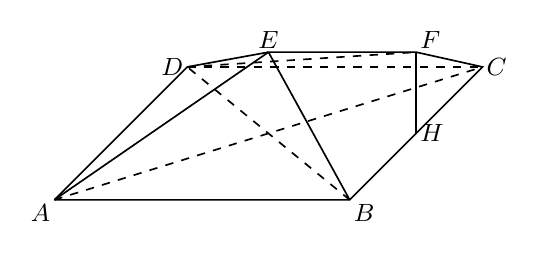
\begin{tikzpicture}[semithick, scale=1.25,
  every node/.style={inner sep=1.2pt, font=\small}]
  \coordinate (A) at (0,0);
  \coordinate (B) at (3,0);
  \coordinate (C) at (4.35,1.35);
  \coordinate (D) at (1.35,1.35);
  \coordinate (E) at (2.175,1.50);
  \coordinate (F) at (3.675,1.50);
  \coordinate (H) at (3.675,0.675);
  % 可见棱
  \draw (A) -- (B) -- (C) -- (F) -- (E) -- (A);
  \draw (A) -- (D) -- (E);
  \draw (B) -- (E);
  \draw (F) -- (H);
  % 被遮挡的棱与辅助线
  \draw[dashed] (D) -- (C);
  \draw[dashed] (A) -- (C);
  \draw[dashed] (B) -- (D);
  \draw[dashed] (D) -- (F);
  % 顶点标注
  \node[below left] at (A) {$A$};
  \node[below right] at (B) {$B$};
  \node[right] at (C) {$C$};
  \node[left] at (D) {$D$};
  \node[above] at (E) {$E$};
  \node[above right] at (F) {$F$};
  \node[right] at (H) {$H$};
\end{tikzpicture}
